\subsection{Configuração da Simulação}

Todos os algoritmos executam em um simulador de eventos discretos \acrotip{VEC} customizado escrito em C++20 com \texttt{simcpp20} e a biblioteca de álgebra linear Armadillo. As redes neurais são treinadas e exportadas usando LibTorch (API C++ do PyTorch). Os cenários de mobilidade são gerados com parâmetros \acrotip{V2X} realistas, com velocidades veiculares de \SI{30}{\kilo\meter\per\hour} a \SI{120}{\kilo\meter\per\hour}, largura de banda de uplink \acrotip{5G} de \SI{20}{\mega\hertz}, sidelink \acrotip{V2V} de \SI{10}{\mega\hertz}, frequência do \acrotip{RSU} $f_{\mathrm{RSU}} = \SI{2}{\giga\hertz}$ e frequência embarcada $f_{\mathrm{loc}} \in [0{,}5;\, 1{,}0]$\,GHz. Os prazos das tarefas seguem uma Gaussiana truncada em $[0{,}05;\, 2{,}0]$\,s; complexidade de CPU $C_j \sim \mathrm{Uniforme}[10^8, 10^{10}]$ ciclos.

\paragraph{Treinamento.} Todos os agentes \acrotip{DRL} são treinados por 400 episódios em cenários com densidade veicular fixa de \SI{10}{tasks\per\second}. Cada episódio de treinamento simula 100 chegadas de tarefas com uma nova realização de mobilidade extraída da mesma distribuição.

\paragraph{Teste.} Após o treinamento, os agentes são avaliados zero-shot em 601~cenários de teste cobrindo cinco regimes de densidade: $\{10, 15, 20, 25, 30\}$~tasks/s. Nenhum aprendizado ou adaptação adicional ocorre durante os testes.

\paragraph{Linhas de base.} Comparamos com: Always-Local (nunca descarrega), Greedy (sempre descarrega ao par \acrotip{V2V} com menor \acrotip{JCT} estimado, uma linha de base oráculo otimista), Greedy-Fair (greedy com restrição de equidade de Jain), Random (descarrega a um par aleatório), SAC-Base (\acrotip{SAC} com vetor de estado bruto de 11 dimensões, sem \acrotip{TOPSIS}), PPO-TOPSIS (\acrotip{PPO} on-policy com o mesmo estado \acrotip{TOPSIS} 6D) e TD3-TOPSIS (\acrotip{TD3} off-policy com o mesmo estado \acrotip{TOPSIS} 6D).

\paragraph{Métricas.}
\begin{itemize}[nosep,leftmargin=*]
  \item \textbf{Taxa de cumprimento de prazo}: fração de tarefas com
        $\mathrm{JCT}_j \le D_j$.
  \item \textbf{\acrotip{SWQ}}:
        $\mathrm{SWQ} = \hat{\tau} \cdot
         \overline{\bigl[(D_j - \mathrm{JCT}_j)/D_j\bigr]}_{\mathrm{sucesso}}$,
        que recompensa o cumprimento do prazo com grande folga.
  \item \textbf{\acrotip{JCT} médio} e \textbf{energia total consumida}.
\end{itemize}

\subsection{Comparação Geral de Desempenho}

A Figura~\ref{fig:performance} e a Tabela~\ref{tab:results} resumem o desempenho agregado em todos os 601~cenários de teste.

\begin{figure}[t]
  \centering
  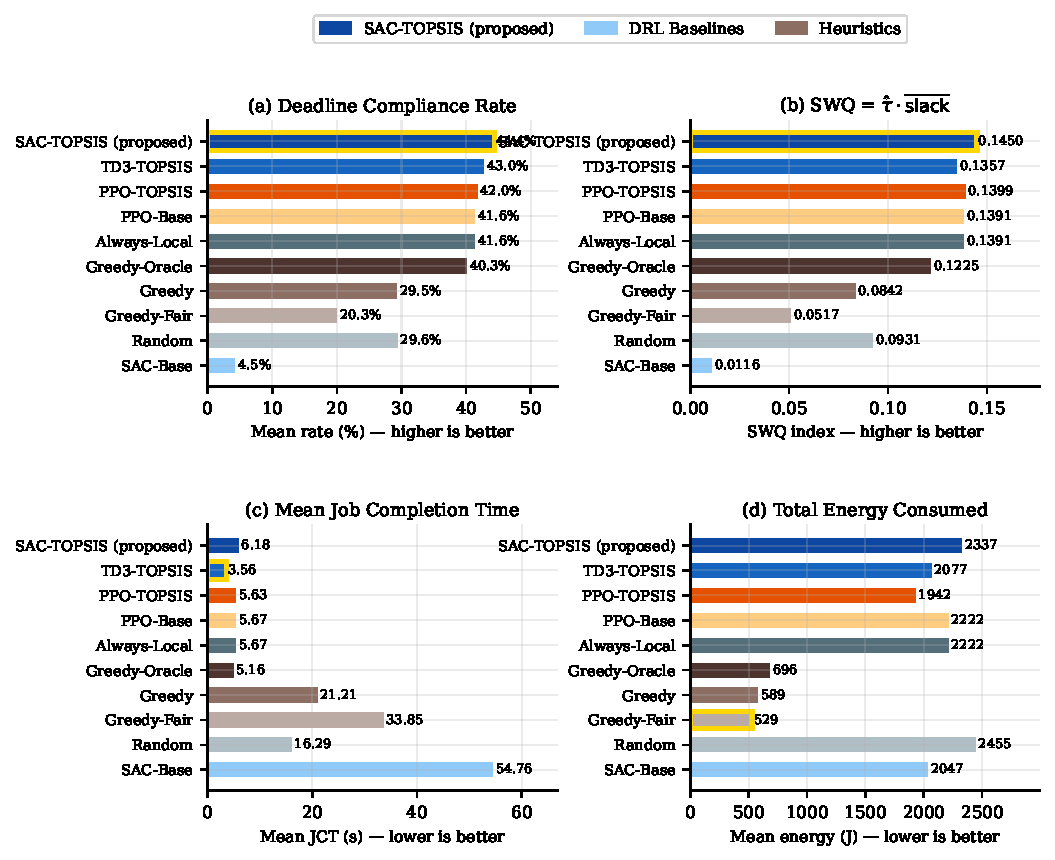
\includegraphics[width=\columnwidth]{images/fig_02_performance.pdf}
  \caption{Comparação de desempenho entre as principais métricas.
           O \acrotip{SAC}-\acrotip{TOPSIS} (azul escuro) alcança a maior taxa de cumprimento de
           prazo e o maior índice \acrotip{SWQ}.
           A borda dourada marca o melhor valor em cada gráfico.}
  \label{fig:performance}
\end{figure}

\begin{table}[t]
\caption{Desempenho agregado em 601~cenários de teste
         (média por cenário, densidades $\{10,15,20,25,30\}$~tasks/s).
         As setas ($\uparrow$) indicam o ganho ao adicionar \acrotip{TOPSIS} a cada
         algoritmo base. Negrito indica o melhor valor \acrotip{DRL}; $\dagger$ indica
         a linha de base oráculo.}
\label{tab:results}
{\small
\addtolength{\tabcolsep}{-3pt}
\begin{tabularx}{\linewidth}{X >{\raggedleft\arraybackslash}X >{\raggedleft\arraybackslash}X >{\raggedleft\arraybackslash}X >{\raggedleft\arraybackslash}X}
\toprule
\textbf{Política} & \textbf{Prazo (\%)} & \textbf{\acrotip{SWQ}} &
\textbf{\acrotip{JCT} (s)} & \textbf{Energia (J)} \\
\midrule
SAC-Base               &  4,47 & 0,0116 & 54,76 & 2047 \\
\acrotip{SAC}-\acrotip{TOPSIS} $\uparrow\mathbf{+39,9}$ & \textbf{44,36} & \textbf{0,1450} & 6,18 & 2337 \\
\midrule
TD3-Base               & 41,62 & 0,1391 &  \textbf{3,53} & 2222 \\
TD3-TOPSIS $\uparrow+1,4$  & 43,01 & 0,1357 &  3,56 & 2077 \\
\midrule
PPO-Base               & 41,61 & 0,1391 &  5,67 & 2222 \\
PPO-TOPSIS $\uparrow+0,3$  & 41,95 & 0,1399 &  5,63 & \textbf{1942} \\
\midrule
Always-Local           & 41,61 & 0,1391 &  5,67 & 2222 \\
\midrule
Greedy-Oracle$^\dagger$ & 40,31 & 0,1225 &  5,16 &  696 \\
Greedy                 & 29,54 & 0,0842 & 21,21 &  589 \\
Greedy-Fair            & 20,26 & 0,0517 & 33,85 &  529 \\
Random                 & 29,61 & 0,0931 & 16,29 & 2455 \\
\bottomrule
\end{tabularx}}
\end{table}

\paragraph{O \acrotip{TOPSIS} melhora consistentemente todas as famílias \acrotip{DRL}.} A Tabela~\ref{tab:results} revela um resultado central deste artigo: parear o \acrotip{TOPSIS} com qualquer algoritmo \acrotip{DRL} testado melhora a taxa de cumprimento de prazo em relação à versão base correspondente. A magnitude do ganho, contudo, varia substancialmente entre as famílias de algoritmos e reflete a interação entre o estado \acrotip{TOPSIS} e a estratégia de exploração de cada algoritmo.

\acrotip{SAC} experimenta a melhoria mais dramática:
o SAC-Base alcança apenas $4{,}47\%$ de cumprimento porque converge para uma
política quase sempre de descarregamento ($94{,}9\%$ \acrotip{V2V}), incorrendo em
atrasos proibitivos de fila quando os vizinhos estão congestionados.
Adicionar o estado \acrotip{TOPSIS} resgata a política para $44{,}36\%$
($\mathbf{+39{,}9}$\,pp), o melhor resultado entre todas as políticas avaliadas.
A representação 6D fornece o sinal semântico, com razões de urgência e ocupações de
fila, necessário para que o \acrotip{SAC} precisa para distinguir decisões de descarregamento benéficas
das prejudiciais.

\acrotip{TD3} já colapsa para always-local em sua forma base ($41{,}62\%$,
idêntico ao Always-Local), pois sua política determinística evita o caminho
arriscado \acrotip{V2V} sem pressão de exploração.
Com o estado \acrotip{TOPSIS}, o \acrotip{TD3} aprende a explorar \acrotip{V2V} oportunisticamente
($23{,}4\%$), elevando o cumprimento para $43{,}01\%$ ($+1{,}4$\,pp) e
alcançando o menor \acrotip{JCT} médio ($3{,}56$\,s) de todas as políticas.

\acrotip{PPO} também colapsa para always-local em sua forma base ($41{,}61\%$)
devido à alta variância do gradiente on-policy.
O estado \acrotip{TOPSIS} proporciona melhora marginal para $41{,}95\%$ ($+0{,}3$\,pp).
O ganho é limitado porque a natureza on-policy do \acrotip{PPO} o impede de explorar
plenamente o estado mais rico, pois a variância nas estimativas de gradiente ainda
empurra a política para a ação local segura, apesar do sinal informativo $s_2$
(vantagem de descarregamento).

No geral, o \acrotip{SAC}-\acrotip{TOPSIS} alcança a maior taxa de cumprimento de prazo
($44{,}36\%$) e \acrotip{SWQ} ($0{,}1450$) entre todas as políticas, incluindo a linha
de base oráculo Greedy ($40{,}31\%$).
Os resultados confirmam que o estado \acrotip{TOPSIS} é o principal motor de
desempenho, e não da escolha do algoritmo \acrotip{DRL}, pois as três famílias se beneficiam,
e as diferenças residuais entre elas são efeitos secundários de seus respectivos
mecanismos de exploração.

\subsection{Generalização Zero-Shot}

A Figura~\ref{fig:generalization} mostra a taxa de cumprimento de prazo em
função da densidade veicular.
O \acrotip{SAC}-\acrotip{TOPSIS} lidera consistentemente em todas as densidades, mantendo $>34\%$
de cumprimento mesmo no regime de congestionamento inédito mais severo
($\SI{30}{tasks\per\second}$), onde o Greedy heurístico cai para apenas $14\%$.
A diferença sobre o Always-Local varia de $+1{,}73$\,pp em 25~tasks/s a
$+4{,}15$\,pp em 10~tasks/s, confirmando que o benefício de aprender uma
política adaptativa é mais pronunciado em menor congestionamento, onde o
descarregamento \acrotip{V2V} oportunista é mais confiável.

\begin{figure}[t]
  \centering
  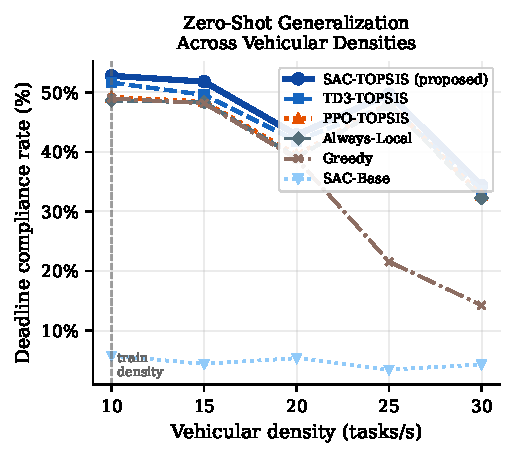
\includegraphics[width=0.75\columnwidth]{images/fig_03_generalization.pdf}
  \caption{Taxa de cumprimento de prazo em função da densidade veicular.
           Todos os agentes foram treinados apenas em 10~tasks/s (linha
           vertical tracejada).
           O \acrotip{SAC}-\acrotip{TOPSIS} (círculos sólidos) supera todas as linhas de base
           consistentemente sem retreinamento específico por densidade.}
  \label{fig:generalization}
\end{figure}

A invariância à escala do vetor de estado 6D é o habilitador fundamental: como $s_3$–$s_4$ são razões relativas ao prazo e $s_5$–$s_6$ são ocupações de fila normalizadas, a política aprendida pelo agente transfere-se diretamente para ambientes com mais ou menos candidatos. O SAC-Base, em contraste, codifica tamanhos absolutos de fila e valores brutos de frequência que perdem seu significado sob mudança de distribuição.

\subsection{Distribuição dos Modos de Execução}

A Figura~\ref{fig:modes} mostra a proporção média de execuções locais, \acrotip{RSU} e
\acrotip{V2V} por política.
O \acrotip{SAC}-\acrotip{TOPSIS} explora o descarregamento \acrotip{V2V} ($25{,}9\%$), que oferece menor
latência que o \acrotip{RSU} quando um veículo par está próximo.
Crucialmente, o módulo \acrotip{TOPSIS} garante que o \acrotip{V2V} seja escolhido apenas quando
oferece uma pontuação \acrotip{TOPSIS} melhor que o \acrotip{RSU}, impedindo a migração de carga
para pares sobrecarregados.

\begin{figure}[t]
  \centering
  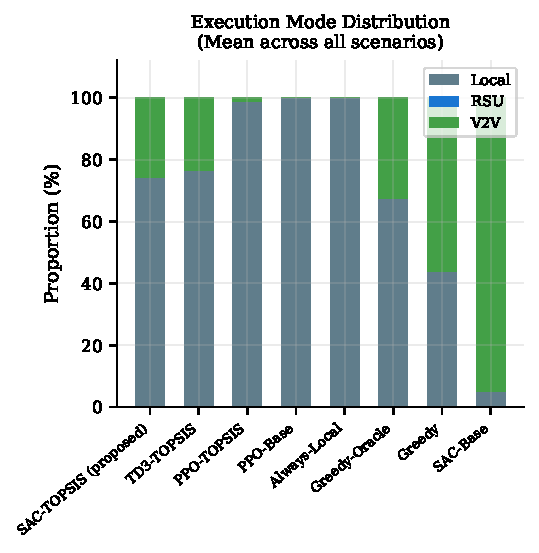
\includegraphics[width=0.75\columnwidth]{images/fig_04_modes.pdf}
  \caption{Distribuição dos modos de execução.
           O \acrotip{SAC}-\acrotip{TOPSIS} equilibra adaptativamente execução local e \acrotip{V2V},
           enquanto o SAC-Base sobrecarrega o \acrotip{RSU} com descarregamentos.}
  \label{fig:modes}
\end{figure}

\subsection{Convergência do Treinamento}

A Figura~\ref{fig:training} compara as curvas de treinamento do \acrotip{SAC}-\acrotip{TOPSIS}, SAC-Base, TD3-TOPSIS e PPO-TOPSIS. Todos os agentes são treinados por $400$ episódios no cenário de 10~tasks/s. \acrotip{SAC}-\acrotip{TOPSIS} e TD3-TOPSIS exibem melhoria de recompensa mais rápida e menor variância que o SAC-Base, confirmando que o estado \acrotip{TOPSIS} fornece um sinal de aprendizado mais informativo. O PPO-TOPSIS converge para um ótimo local com menor recompensa média, consistente com sua política always-local no tempo de teste.

\begin{figure}[t]
  \centering
  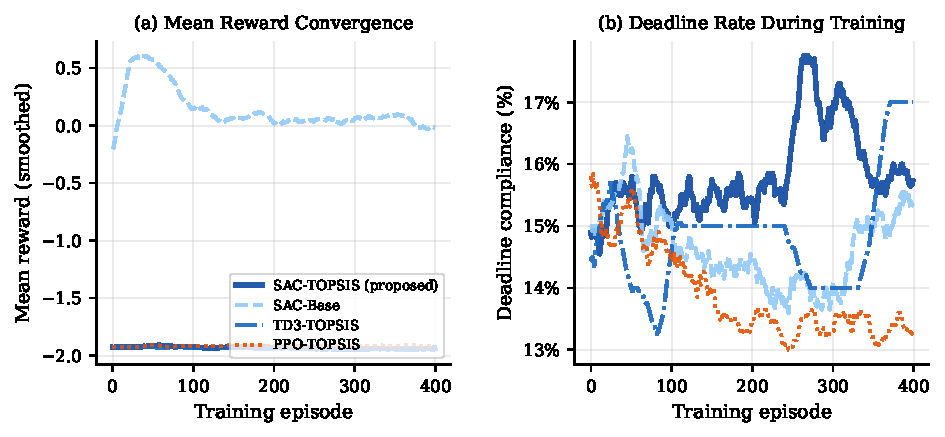
\includegraphics[width=\columnwidth]{images/fig_05_training.pdf}
  \caption{Convergência do treinamento ao longo de 400 episódios.
           (a)~Recompensa média (suavizada com janela de 20 episódios);
           (b)~taxa de cumprimento de prazo durante o treinamento.
           O \acrotip{SAC}-\acrotip{TOPSIS} alcança convergência estável em ambas as métricas.}
  \label{fig:training}
\end{figure}

\subsection{Estudo de Ablação: \acrotip{TOPSIS} como Primitiva Universal de Engenharia de Estado}
\label{sec:ablation}

A Figura~\ref{fig:ablation} apresenta uma ablação cross-família na qual cada algoritmo \acrotip{DRL} é avaliado com seu estado base bruto e com o estado \acrotip{TOPSIS} 6D, mantendo todos os demais hiperparâmetros idênticos. As setas que anotam cada par quantificam o ganho atribuível exclusivamente à mudança de representação de estado.

Três achados se destacam. Primeiro, o ganho é monótono, pois o \acrotip{TOPSIS} nunca prejudica nenhum algoritmo. Segundo, o ganho é maior para a política base mais instável (SAC-Base colapsa, \acrotip{SAC}-\acrotip{TOPSIS} recupera), o que confirma que o estado \acrotip{TOPSIS} resolve o problema de colapso de representação em vez de apenas ajustar uma política já razoável. Terceiro, o ganho é agnóstico ao algoritmo, pois mesmo o \acrotip{TD3}, que tem uma política base bem comportada (ainda que conservadora), melhora $+1{,}4$\,pp após a mudança de estado. Este último ponto é fundamental, pois mostra que o estado \acrotip{TOPSIS} carrega informação útil além do que qualquer algoritmo base pode inferir a partir de observações brutas, e que essa informação é explorável por diferentes paradigmas de aprendizado.

\begin{figure}[t]
  \centering
  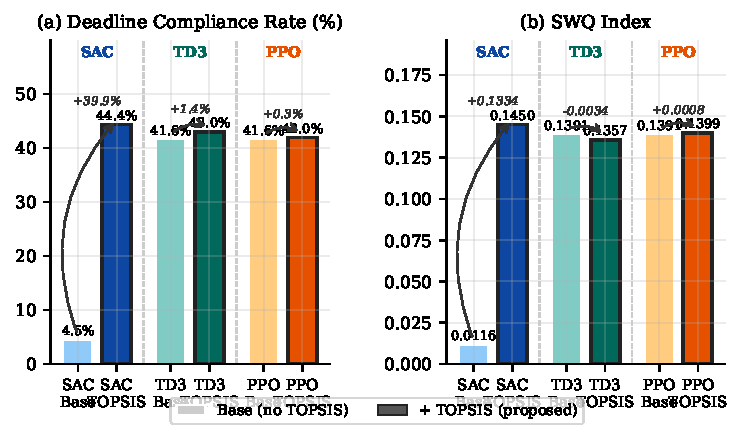
\includegraphics[width=\columnwidth]{images/fig_06_ablation.pdf}
  \caption{Ablação cross-família: Base (sem \acrotip{TOPSIS}, barras mais claras) vs.\
           +\acrotip{TOPSIS} (barras mais escuras com borda preta) para \acrotip{SAC}, \acrotip{TD3} e \acrotip{PPO}.
           As setas curvas mostram o ganho ao adicionar \acrotip{TOPSIS} a cada família.
           O ganho é consistente em todas as famílias, confirmando que a
           compressão de estado \acrotip{TOPSIS} é um motor de desempenho universal.}
  \label{fig:ablation}
\end{figure}

\subsection{Ablação Interna do \acrotip{SAC}: Decomposição Causal}
\label{sec:sac_ablation}

Para entender quais escolhas de projeto dentro do \acrotip{SAC}-\acrotip{TOPSIS} mais contribuem para seu desempenho, conduzimos uma ablação refinada na qual cada variante adiciona exatamente um componente em relação ao SAC-Base. A Tabela~\ref{tab:sac_ablation} e a Figura~\ref{fig:sac_ablation} resumem os resultados.

\begin{table}[t]
\caption{Ablação interna do \acrotip{SAC}. Cada linha adiciona uma escolha de projeto
         sobre o SAC-Base. $\Delta$ é o ganho na taxa de prazo em relação ao
         SAC-Base.}
\label{tab:sac_ablation}
{\small
\addtolength{\tabcolsep}{-4pt}
\begin{tabularx}{\linewidth}{X >{\centering\arraybackslash}X >{\raggedleft\arraybackslash}X >{\raggedleft\arraybackslash}X}
\toprule
\textbf{Variante} & \textbf{Mudança} & \textbf{Prazo} & $\boldsymbol{\Delta}$ \\
\midrule
SAC-Base  & — (base)                        &  4,47\% & —      \\
SAC-A1    & Ação binária                     & 38,59\% & +34,1  \\
SAC-R1    & Recompensa                      & 37,64\% & +33,2  \\
SAC-S1    & Estado compacto                 & 28,32\% & +23,8  \\
SAC-T1    & \acrotip{TOPSIS} 3-ac           & 32,10\% & +27,6  \\
\acrotip{SAC}-\acrotip{TOPSIS}& Completo            & \textbf{44,36}\% & \textbf{+39,9}  \\
\bottomrule
\end{tabularx}}
\end{table}

\begin{figure}[t]
  \centering
  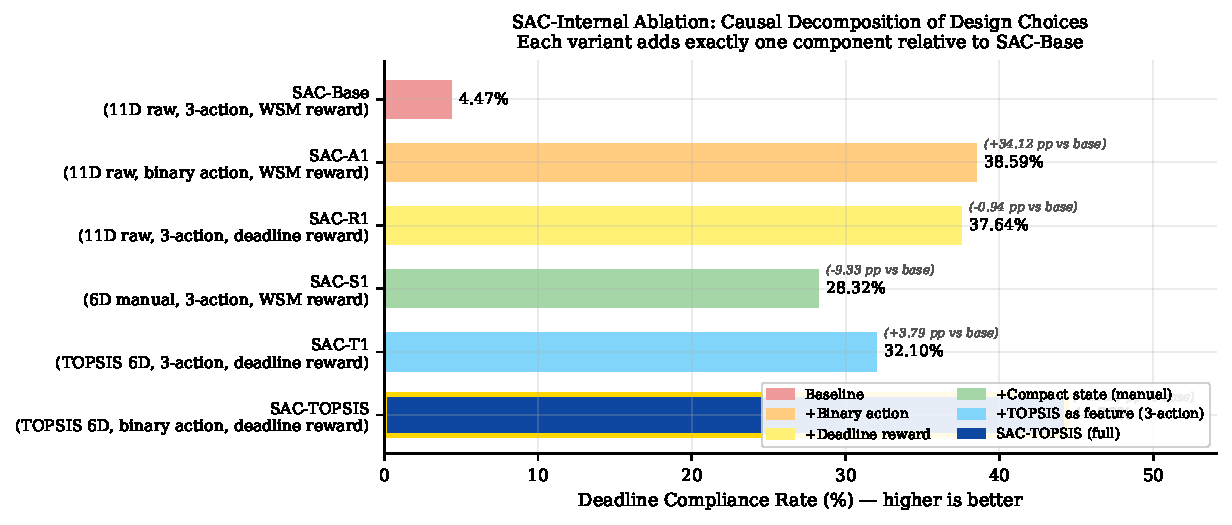
\includegraphics[width=\columnwidth]{images/fig_07_sac_ablation.pdf}
  \caption{Decomposição causal interna do \acrotip{SAC}.
           Cada barra corresponde a uma variante que isola uma escolha de
           projeto.
           Todos os ganhos são reportados em relação ao SAC-Base ($4{,}47\%$).
           O \acrotip{SAC}-\acrotip{TOPSIS} completo combina os três componentes e alcança a maior
           taxa de cumprimento.}
  \label{fig:sac_ablation}
\end{figure}

Três perspectivas complementares emergem dessa decomposição.

\begin{enumerate}[label=(\arabic*),leftmargin=*]
  \item A ação binária é a maior alavanca individual (+34,1\,pp, SAC-A1). Reduzir o espaço de ações de três classes (LOCAL/\acrotip{RSU}/\acrotip{V2V}) para uma decisão binária (LOCAL vs.\ melhor descarregamento rank-1) resolve em grande parte o colapso do SAC-Base. Sem \acrotip{TOPSIS}, o agente ainda deve avaliar os candidatos com base em características brutas, mas a simplificação da fronteira de decisão já impede a política degenera sempre-\acrotip{V2V}.
  
  \item A modelagem de recompensa ciente de prazo é igualmente crítica (+33,2\,pp, SAC-R1). Substituir a recompensa do Método da Soma Ponderada (\acrotip{WSM}) pela recompensa contínua proporcional ao prazo da Equação~\eqref{eq:reward} fornece um sinal de gradiente mesmo no regime de falha, permitindo que o agente aprenda a minimizar o atraso em vez de apenas evitá-lo. Esse ganho é independente da representação de estado, demonstrando que a engenharia de recompensa é uma contribuição autônoma.
  
  \item O estado \acrotip{TOPSIS} proporciona ganhos compostos sobre qualquer componente isolado. O SAC-S1 mostra que compactar o estado para 6D manualmente (sem \acrotip{TOPSIS}) já rende $+23{,}8$\,pp sobre o SAC-Base, confirmando que a engenharia de features importa. O SAC-T1 mostra que usar o \acrotip{TOPSIS} para construir o estado 6D (em vez de features ad-hoc) eleva isso para $+27{,}6$\,pp, mesmo quando o espaço de ações ainda tem 3 classes. O \acrotip{SAC}-\acrotip{TOPSIS} completo, que combina o estado \acrotip{TOPSIS} com a ação binária e a recompensa de prazo, alcança $+39{,}9$\,pp, mais que qualquer componente individual, confirmando que as três escolhas de projeto são sinérgicas em vez de meramente aditivas.
\end{enumerate}
